\basicheader
\usepackage[ngerman]{babel}
\usepackage{colortbl}
\usepackage{longtable}
\usepackage[sfdefault,tabular,scaled=.9]{FiraSans}
\usepackage[lining,scaled=.9]{FiraMono}
\usepackage[mathrm=sym]{unicode-math}
\usepackage[Scale=.9]{firamath-otf}
\usepackage{luatexbase}
\usepackage{microtype}
\usepackage[hang,symbol,multiple]{footmisc}
\usepackage{tikz}
\usepackage{xstring}
\usepackage{enumitem}
\usepackage{xcolor}

\input graphdrawing.tex

\input translation-\ifcsdef{TemplateLanguage}{\TemplateLanguage}{de}.tex
\fancyheadoffset[roh,reh]{.667em}

% Logo
\definecolor{highlightcolor}{HTML}{c20e1a}
\def\logo{
\begin{tikzpicture}
    \node[anchor=east] (pic) at (0, 0) {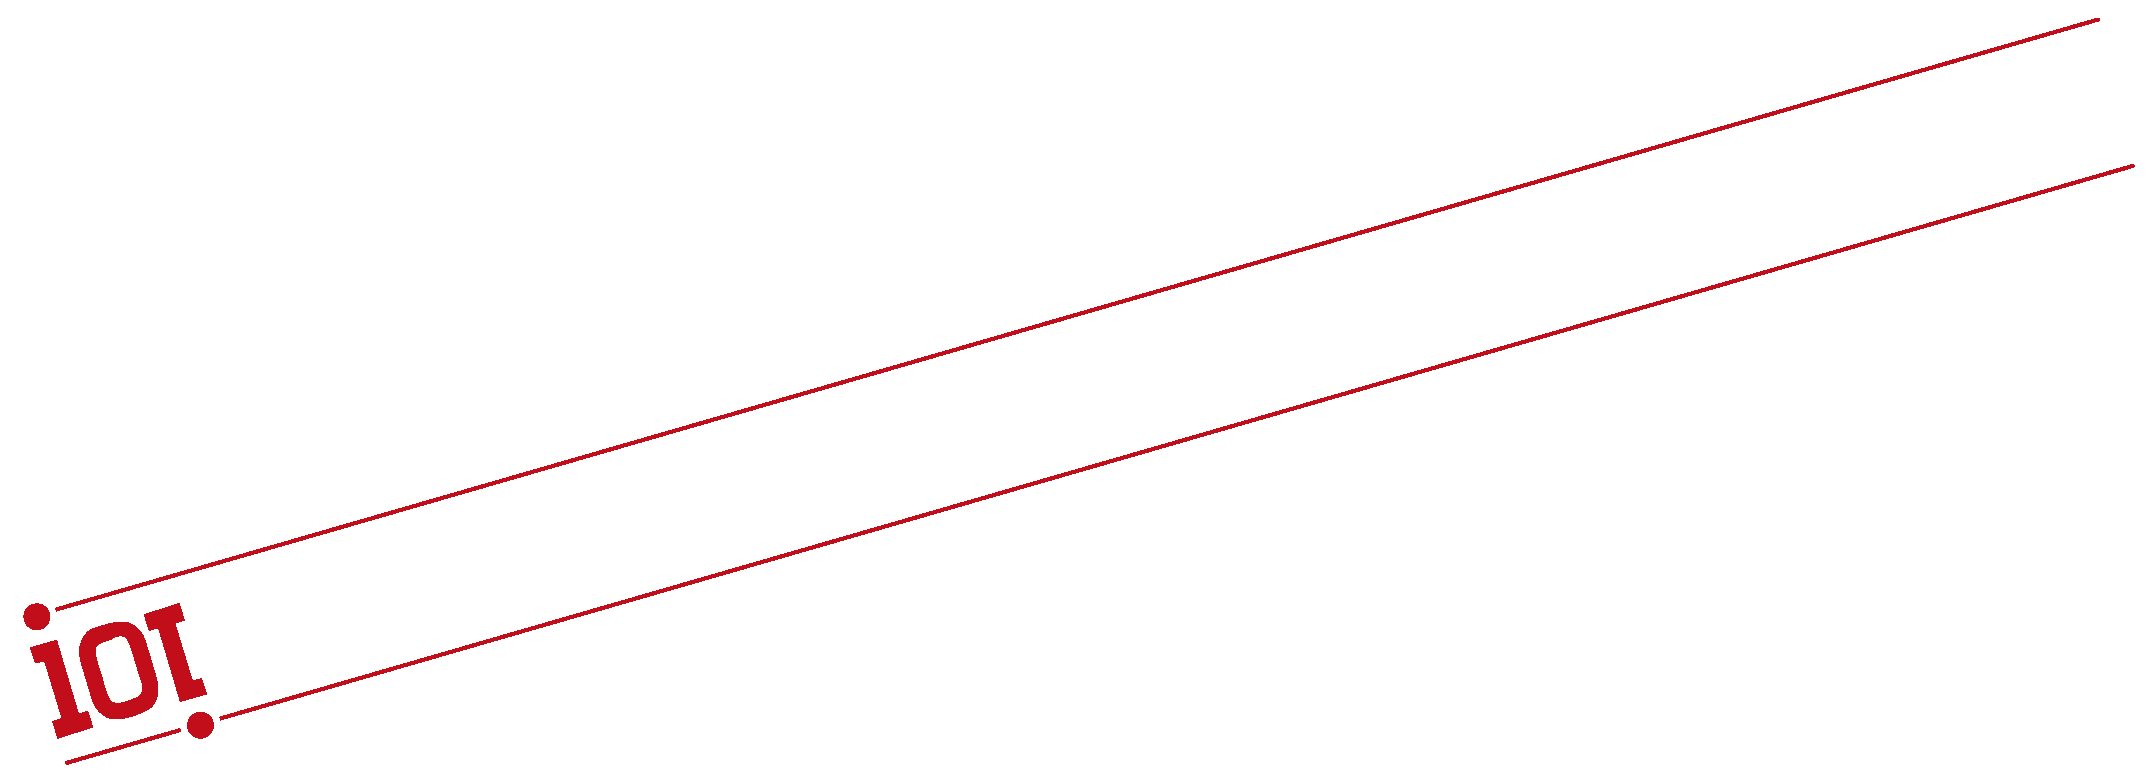
\includegraphics[scale=.45]{logo.eps}};
    \node[white!40!black,anchor=west,align=left, outer xsep=1em] (A) at (1em,0)
        {{\bfseries\contestname}\\\tTask:\enspace\bfseries\taskname};
    \draw[highlightcolor,very thick] (A.north west) -- (A.south west);
\end{tikzpicture}
}
\rhead{\logo} \lhead{}


\makeatletter
\def\inputwidth{.4705\textwidth}
\def\outputwidth{.4705\textwidth}

% Subtask headings
\def\sthelper#1#2{{\sffamily\bfseries \tSubtask\ #1 ($\symbf{#2}$ \IfInteger{#2}{\ifnum#2=1\tPoint\else\tPoints\fi}{\tPoints}).\enspace}}
\newcount\stcount
\stcount=0
\def\st@sk#1{\setbox0=\hbox{\sthelper{9}{99}}\global\advance\stcount by 1 \par\ifdim\lastskip<\smallskipamount\removelastskip\smallskip\fi\noindent\hangindent=\wd0 \hangafter=1%
\setbox1=\hbox{\sthelper{\the\stcount}{#1}\hss}%
\ifdim\wd1>\wd0\box1\else\hbox to \wd0{\unhbox1\hss}\fi\ignorespaces}
\def\subtask{\count1=\stcount \advance\count1 by 1 \st@sk{\subtaskpoints{\the\count1}}}


% Constraints
\def\currconstraint#1{\scopedconstraint{\the\stcount}{#1}}
\def\currconstraints{\@ifstar{\currconstraint{@ll*}}{\currconstraint{@ll}}}
\def\currconstraintupper#1{\scopedconstraintupper{\the\stcount}{#1}}
\def\currconstraintlower#1{\scopedconstraintlower{\the\stcount}{#1}}
\def\currconstraintvalue#1{\scopedconstraintvalue{\the\stcount}{#1}}


% Sample interaction for interactive tasks
\def\programcolumnwidth{3.55cm}
\def\returncolumnwidth{3cm}
\def\explanationcolumnwidth{8.025cm}
\begingroup
\catcode`\ǁ=4
\catcode`\& =\active%
\gdef\@ctivateAMP{\def&{ǁǁ}}
\endgroup
\newenvironment{interactiontable}{\begingroup%
\catcode`\& =\active%
\@ctivateAMP%
\par\medskip%
\begin{tabular}{>{\cellcolor[gray]{.9}}p{\programcolumnwidth}@{\hskip0pt}p{.52cm}@{\hskip0pt}>{\cellcolor[gray]{.9}}p{\returncolumnwidth}@{\hskip0pt}p{.52cm}@{\hskip0pt}>{\cellcolor[gray]{.9}\sffamily\hangindent=1.25em\hangafter=1\raggedright\arraybackslash}p{\explanationcolumnwidth}}
\hline
\multicolumn{1}{|c}{\cellcolor{white}\sffamily\tProgram}&&\multicolumn{1}{c}{\sffamily \tReturn}&&\multicolumn{1}{c|}{\sffamily\tExplanation}\\\hline
\noalign{\smallskip}%
}{\end{tabular}\endgroup\par\medskip}


% Sample for (standard) batch tasks
\setlength{\LTpost}{\medskipamount}
\def\myc@ption#1#2#3{\noalign{\bfseries\large #3}}
\def\showcases{\removelastskip\par\bigskip\begingroup%
% This is evil: we hijack LT@makecaption to force longtable to place the heading
% same page as the table...
\let\LT@makecaption=\myc@ption
\begingroup%
\microtypesetup{activate=false}%
\testcasetable%
\endgroup%
\endgroup}


% Limits
\def\showlimits{\sheading{\tLimits}%
\tTime: \timelimit\\
\tMemory: \memlimit}


% Feedback [[deprecated]]
\def\feedbackheading{\sheading{\tFeedback}}
\def\nofeedback{\feedbackheading \tNofeedback}
\def\partialfeedback{\feedbackheading \tPartialfeedback}
\def\fullfeedback{\feedbackheading\def\feedbackmode{\ifrestricted\emph{restricted feedback}\else\emph{full feedback}\fi} \tFullfeedbackGeneral\
\ifrestricted
\tRestrictedfeedbackPrecise
\else
\tFullfeedbackPrecise
\fi}
\def\tokenfeedback{\feedbackheading \tTokenFeedback
\ifrestricted
\tTokenRestrictedFeedback
\fi}
\let\dummyfeedack=\relax
\def\showfeedback{\PackageWarning{lg-template}{We've been using the same feedback settings for years; are you really sure you want to include them in the statement?}\csname\feedback feedback\endcsname}


% Scoring [[deprecated]]
\def\scoringheading{\sheading{\tScoring}}
\def\IOIXIIIscoring{\scoringheading \tScoringFromIOIXIII}
\def\IOIXVIIscoring{\scoringheading \tScoringFromIOIXVII}
\def\IOIXscoring   {\scoringheading \tScoringFromIOIX}
\def\showscoring{\PackageWarning{lg-template}{We've been using the same scoring mode for years; are you really sure you want to include it in the statement?}\csname\scoring scoring\endcsname}


% all of the above
\def\standardpart{\showcases\showlimits}
\makeatother


% math settings
\def\setmymathdims{\global\Umathsubshiftdown\textstyle=2.5pt%
\global\Umathsubshiftdrop\textstyle=2.5pt%
\global\Umathsubtopmax\textstyle=4pt%
\global\Umathsupshiftup\textstyle=3.75pt%
\global\Umathopopenspacing\textstyle=225mu
\global\Umathsubshiftdrop\displaystyle=3pt%
\global\Umathsubshiftdown\displaystyle=3pt%
\global\Umathsubtopmax\displaystyle=3pt%
\global\Umathsupshiftdrop\displaystyle=4pt%
\global\Umathsupshiftup\displaystyle=4pt%
\global\Umathopopenspacing\textstyle=2.25mu}
\AtBeginDocument{\everymath{\setmymathdims}\setbox0=\hbox{$ $}\setmymathdims}


% nice items
\setlist[itemize,1]{label={\begin{tikzpicture}
    \useasboundingbox (0,-1.25pt) rectangle (5pt,4.25pt);
    \fill[highlightcolor] (0,0)--(0,4pt)--(4pt,4pt)--(4pt,0)--cycle;
\end{tikzpicture}}}


% ensure all subtasks appear in the statement...
\AtEndDocument{\ifnum\stcount=\numsubtasks\else\PackageError{lg-template}{Not all subtasks are contained in the task statement!\MessageBreak You should call \protect\subtask\space (or \protect\st) precisely as often as there are subtasks, not counting the public one. If for some reason you do not want to do this, you can call \protect\flushsubtasks\space after all calls to \protect\subtask\space and \protect\st}{You should call \protect\subtask\space (or \protect\st) precisely as often as there are subtasks, not counting the public one. If for some reason you do not want to do this, you can call \protect\flushsubtasks\space after all calls to \protect\subtask\space and \protect\st}\fi}

% ... or not (only use this if you know what you are doing)
\def\flushsubtasks{\global\stcount=\numsubtasks}